\documentclass[11pt]{article}
\usepackage{amsmath,amssymb,color,hyperref,graphicx,pdfsync}
\usepackage{svn}
\SVN $Date$
\SVN $Revision$
\SVN $Author$
\SVN $HeadURL$
\newcommand\revisioninfo{\centerline{\textcolor{blue}{Revision: \SVNRevision ; Last changed by \SVNAuthor\ on \SVNDate .}}}

\graphicspath{{Figures/}}

\textwidth 5.5 truein
\oddsidemargin .5 truein
\evensidemargin .5 truein
\topmargin -.5 truein
\textheight 8.5in

\def\question#1{\textcolor{red}{\bf Question:} #1}

%\def\code#1{{\ttfamily #1}}
\def\class#1{{\bf #1}} % \bfseries
\def\fn#1{{\tt #1}} % \ttfamily
\def\virtualfn#1{{\it #1}} % \itshape

\def\cmd#1{{\bfseries #1}}
\def\ttcmd#1{{\ttfamily\cmd{#1}}}
\def\arg#1{\textit{#1}}
\def\optarg#1{[\arg{#1}]}
% \def\<#1>{\leavevmode\hbox{$\langle$#1\/$\rangle$}} % syntactic quantity
% \def\[#1]{\leavevmode\hbox{$\langle$#1\/$\rangle$}} % optional argument
% \def\spc{\<\small SPACE>}
% \def\return{\textit{Return}}
% \def\control{\textit{Control}}
% \def\meta{\textit{Meta}}
% \def\esc{{\small ESC}}

% % for verbatim entries (from Knuth's manmac)
% \chardef\other=12
% \def\ttverbatim{\begingroup \catcode`\\=\other \catcode`\{=\other
%   \catcode`\}=\other \catcode`\$=\other \catcode`\&=\other
%   \catcode`\#=\other \catcode`\%=\other \catcode`\~=\other
%   \catcode`\_=\other \catcode`\^=\other
%   \obeyspaces \obeylines \tt}
% \newskip\ttglue
% \ttglue=.5em plus.25em minus.15em
% {\catcode`\|=\active \obeylines
% \gdef|{\ttverbatim\spaceskip=\ttglue\let^^M=\ \let|=\endgroup}}
% \catcode`\|=\active

% % for command line displays (from Knuth's manmac)
% \outer\def\begintt{$$\let\par=\endgraf \ttverbatim \parskip=0pt
%   \catcode`\|=0 \rightskip=-5pc \ttfinish}
% {\catcode`\|=0 |catcode`|\=\other % | is temporary escape character
%   |obeylines % end of line is active
%   |gdef|ttfinish#1^^M#2\endtt{#1|vbox{#2}|endgroup$$}}

\begin{document}

\title{Design document for Immersed Boundary Projection Method (IBPM)}
\author{Clancy Rowley}
\date{\revisioninfo}
\maketitle

\section{Purpose of this document}
This document describes the high-level design of a code to implement the fast (multiple-grid) Immersed Boundary Projection Method (IBPM) of Colonius and Taira \cite{ColTai-07}.  Here we give a high-level overview of the classes planned, interactions between them, and their public interfaces.  Where appropriate, we describe ideas for possible implementations, but for the most part we leave implementation to the detailed class design.

This document is {\em not} intended to be a ``living'' document that evolves as changes are made to the code (although such modifications would of course be appropriate should major changes or additions to the code be undertaken).  The intent is for the ``living'' documentation to be contained within the code itself, to be extracted using Doxygen.

\section{History and design approach}

\subsection{Previously used code and its limitations}
Prior to the development of the code described in this document, we have been using an implementation of the Immersed Boundary Projection Method (IBPM) written by Colonius and Taira, using Fortran 90.  However, because of the complexity and the tight coupling of the Fortran implementation, this code has become difficult to maintain.  For instance, we wished to change the timestepper, from a second-order Adams-Bashforth/Crank-Nicolson scheme (a two-step scheme) to a Runge-Kutta/Crank-Nicolson scheme, both for improved timestep restrictions, and to sidestep certain issues with a multi-step scheme, when used for adjoint simulations, eigenvalue solvers, and the like.  However, the Fortran~90 code is tightly coupled, making extensive use of global or global-like data (publicly accessible module data), and even making such an apparently simple modification would require major surgery (in particular, to the long routine {\tt operators.f90::advance}, as well as {\tt myfft.f90::setup\_fft}).  Such modifications throughout the code would be error prone, and it would be difficult to switch between integrators, should one wish to go back to Adams-Bashforth, or try other timesteppers.  

Furthermore, the Fortran code has already become rather unwieldy, with flags for different modes of operation, such as solving the linearized or adjoint equations.  This implementation using flags has proven error-prone as well, since the switching logic is distributed throughout the code, and future modifications require a thorough knowledge of many parts of the code.

There are many other smaller reasons for revamping the design of this previous code, for instance improving the mechanism for reading input files, specifying geometries, and especially specifying the motion of moving bodies.  But another major reason for redesign is to facilitate testing, and in particular automated testing at the level of individual routines or groups of routines.  The extensive use of global-like data makes such automated testing difficult or impossible, further hampering the maintainability of the code as new features are added.

\subsection{Overview of design approach}
In order to overcome the difficulties described above, an object-oriented design approach is used here.  The reasons for this are as follows:
\begin{itemize}
	\item Using inheritance eliminates the need to have switching logic distributed throughout the code, for instance for different versions of timesteppers, or different equations of motion.  Furthermore, related operations such as nonlinear, linear, and adjoint versions of the equations of motion can inherit common portions from a parent class, avoiding the need to duplicate large sections of code, which creates more maintenance problems.
	\item Using classes to store private data needed only by certain portions of the code (such as evaluating terms in the Navier-Stokes equations) encapsulates these algorithms, and avoids the need for global-like data, leading to many advantages.  In particular, if one is simply using these routines, one can safely ignore their implementation, focusing only on the interfaces.
	\item Establishing clean, sensible interfaces allows one to test these routines much more easily, and in an automated fashion, which would greatly facilitate debugging, and ensure that new bugs are not introduced when new functionality is added.
\end{itemize}

A key point is to separate {\em interface} from {\em implementation}, so that code that provides a service (i.e., provides a particular implementation) is cleanly separated (via the interface) from code that uses this service.  In this way, the implementation of various portions of the code can evolve without affecting the rest of the code, as long as the interface remains consistent.

\subsection{What the code does}
For details of the numerical method this code solves, see~\cite{ColTai-07}.  Here, we give only a brief overview.

\paragraph{Immersed boundary method}
The Navier Stokes equations are solved in two dimensions, using a streamfunction-vorticity formulation, and a finite-volume method.  Thus, fluxes are defined on cell edges, and scalars such as pressure and vorticity (circulation about one cell) are defined at cell centers.

Let $q$ denote the (vector-valued) velocity flux, $\psi$ the streamfunction, and $\gamma$ the circulation about a cell.  The no-slip boundary condition at the surface of an object are imposed by delta-function forces at the boundary locations, and $f$ is a vector of these force values.  The equations to be solved are given as (22) in~\cite{ColTai-07}:
\begin{align}
	\frac{d\gamma}{dt} + C^TE^T\tilde f &= -\beta C^TC\gamma + C^T\mathcal{N}(q) + bc_\gamma
	\label{eq:navier_stokes}\\
EC(S\Lambda^{-1}S)\gamma + bc_s &= u_B.
\label{eq:no_slip}
\end{align}
The first equation is the momentum equation, and the second equation is a constraint representing the no-slip condition, so that velocities at the boundary points match prescribed velocities~$u_B$. The discrete operators in the above equation are described in the table below, and $\beta=1/(Re\delta^2)$, where $\delta$ is the grid spacing.  \begin{center}
\begin{tabular}{ccp{3.5in}}
Operator & Maps & Definition\\
$C$ 	& $\psi\mapsto q$ & curl of a scalar\\
$C^T$ 	& $q\mapsto \gamma$ & curl of a vector in 2d\\
$S$ 	& $\gamma\mapsto\hat\gamma$ & discrete sin transform\\
$-C^TC$	& $\gamma\mapsto\gamma$ & Laplacian, analogous to $\triangle u = \nabla(\nabla\cdot u) - \nabla\times\nabla\times u$\\
$\Lambda$	& $\hat\gamma\mapsto\hat\gamma$ & eigenvalues of Laplacian\\
$E$ 	& $q\mapsto u_B$ & restriction of fluxes everywhere to velocities at boundary\\
$E^T$	& $f\mapsto q$ & regularization of forces at boundary points to fluxes everywhere
\end{tabular}
\end{center}
where $u_B$ is a vector of velocities at boundary points.  The discrete Laplacian $C^TC$ is diagonalized by the discrete sin transform~$S$, and its eigenvalues are known analytically.  Since $\triangle\psi =\gamma$, we have
\begin{equation}
	\psi = S\Lambda^{-1}S\gamma + bc.
\end{equation}
To retrieve the fluxes $q$ from the streamfunction~$\psi$, we need to add in a (prescribed) potential flow solution~$q_\text{pot}$ as well as a boundary term $bc_q$, so we have
\begin{equation}
	q = C\psi + q_\text{pot} + bc_q.
\end{equation}

\paragraph{Time discretization}
Equation~(\ref{eq:navier_stokes}--\ref{eq:no_slip}) are stepped forward in time using a projection method, as follows.  For instance, discretizing the linear terms of (\ref{eq:navier_stokes}) using Crank-Nicolson (trapezoidal rule), and the nonlinear terms using explicit Euler, one obtains
\begin{align}
	\left(1+\frac{\beta\Delta t}{2}C^TC\right)\gamma^{n+1} + \Delta t C^TE^Tf &= \left(1 - \frac{\beta\Delta t}{2}C^TC\right)\gamma^n + \Delta t C^T \mathcal{N}(q^n) + bc_\gamma \label{eq:timestepper}\\
	EC(S\Lambda^{-1}S)\gamma^{n+1} &= u_B - bc_s.
\end{align}
These equations are of the form
\begin{equation}
	\begin{bmatrix}
		\mathcal{A} & \mathcal{C}\\\mathcal{B} & 0
	\end{bmatrix}
	\begin{bmatrix}
		\gamma^{n+1}\\ f
	\end{bmatrix}
	=
	\begin{bmatrix}
		a\\b
	\end{bmatrix}
\label{eq:constrained}
\end{equation}
where
\begin{align}
	\mathcal{A} &= 1 + \frac{\beta\Delta t}{2}C^TC\\
	\mathcal{B} &= \Delta t C^TE^T\\
	\mathcal{C} &= ECS\Lambda^{-1}S\\
	a &= \left(1-\frac{\beta\Delta t}{2}C^TC\right)\gamma^n + \Delta t C^T\mathcal{N}(q^n) + bc_\gamma\\
	b &= u_B - bc_s
\end{align}

\paragraph{Projection method}
We solve the constrained equation~(\ref{eq:constrained}) using the following algorithm:
\begin{equation}
\begin{aligned}
	\mathcal{A}\gamma^* = a\\
	\mathcal{BA}^{-1}\mathcal{C}f = \mathcal{B}\gamma^* - b\\
	\gamma^{n+1} = \gamma^* - \mathcal{A}^{-1}\mathcal{C}f
\end{aligned}
\label{eq:projection_alg}
\end{equation}
Since the matrix $\mathcal{A}$ is easily invertible using a sin transform, one may solve the first equation easily.  The second equation is rather small ($\text{\#forces} \times \text{\#forces}$), and furthermore the matrix on the left-hand-side is symmetric, since $A$ and $C^TC$ have the same eigenvectors.  When the boundary conditions are fixed (stationary bodies), then this matrix is constant in time, and so may be LU decomposed (e.g. using a Cholesky decomposition) once beforehand, and solved rapidly at each timestep.  When the boundary conditions vary in time, then $E$ changes at each step, and a direct solve is not as efficient as an iterative solve, such as a conjugate-gradient method (for symmetric matrices).

In the design below, we decouple the algorithm for the timestepper~(\ref{eq:timestepper}) from the algorithm (\ref{eq:projection_alg}) for solving equation~(\ref{eq:constrained}).

\section{Classes}
In this section, we give a high-level description of the classes involved.  A diagram showing the main classes and their collaborations is shown in Figure~\ref{fig:class_diagram}.  Below, we discuss each of these and their interfaces in more detail.

\begin{figure}
\centering
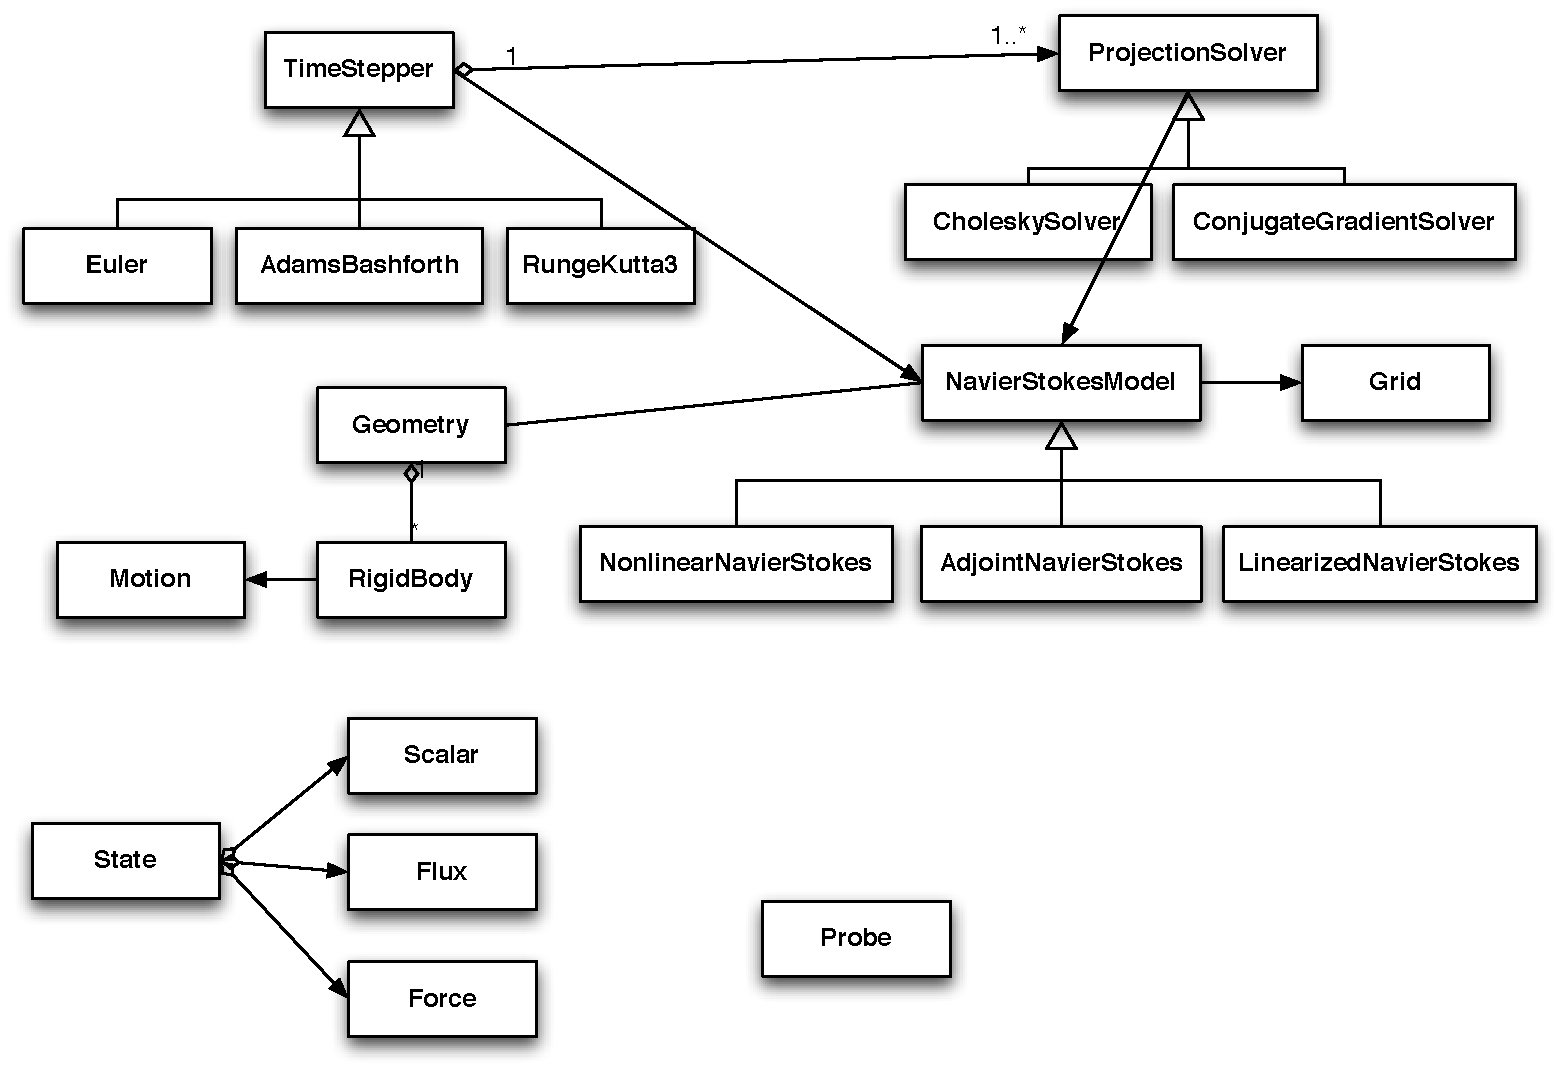
\includegraphics[width=0.95\linewidth]{IBFSDesign}
\caption{Diagram of classes and their collaborations.}
\label{fig:class_diagram}
\end{figure}

\subsection{TimeStepper}
Abstract class collecting routines and data needed to step a solution forward in time.

A \class{TimeStepper} instance has a method \fn{advance} that takes a \class{State}, and computes the value at the next timestep, overwriting the values passed in.  The instance has a pointer to a model (of type \class{NavierStokesModel}), which contains information about the \class{Grid} and \class{Geometry}, as well as the equations to be solved (e.g., \class{LinearNavierStokes}, \class{AdjointNavierStokes}), and instantiates its own \class{ProjectionSolver} as appropriate, for solving the projection step of the equations.  For instance, for a stationary body, the \class{CholeskySolver} should be used, and for moving bodies, for which the projection step in (\ref{eq:projection_alg}) varies at each timestep, an iterative solver such as the \class{ConjugateGradientSolver} is needed.

Note that \class{TimeStepper} is an abstract class, and cannot be instantiated directly.  One of its subclasses must be instantiated.

\paragraph{Interface}
\begin{description}
	\item \fn{TimeStepper}(NavierStokesModel model)\\
		Constructor.  Setup all routines necessary to use \virtualfn{advance}().
	\item \fn{\~\null TimeStepper}()\\
		Destructor.
	\item void \virtualfn{advance}(State x)\\
	 	Advance the state x forward one step, overwriting with the new value.  The governing equations are in the form
	\begin{align}
		\frac{dx}{dt} + Cf &= Lq + N(q)\\
		Bq &= b
	\end{align}
	where the operators in this equation are defined in the associated instance of \class{NavierStokesModel}.  Pure virtual function: subclasses must override this.
	\item Scalar \virtualfn{Ainv\_times}(Scalar g)\\
		Compute\ldots
	\item \virtualfn{B\_times}()\\
		Compute\ldots
	\item \virtualfn{C\_times}()\\
		Compute\ldots
\end{description}

\question{Subclasses should define three routines that can be provided to a \class{ProjectionSolver} instance (that return $\mathcal{A}^{-1}$, $\mathcal{B}$, and $\mathcal{C}$ acting on a vector).  How can a subclass define such a routine and pass it?  Can one pass methods of an object as parameters to a constructor for \class{ProjectionSolver} instance?  If so, do they need to be public, or can they be protected? (Do the two classes need to be friends?)  Would it make sense to define another class \class{ProjectionRoutines} that contains these three routines as methods?  Or just pass an entire \class{TimeStepper} object to the \class{ProjectionSolver}?}

\paragraph{Implementation}
The functionality of the projection step~(\ref{eq:projection_alg}) is contained in the \class{ProjectionSolver}, so the only portion derived classes need to implement when overriding \virtualfn{advance} is a description of the timestepper as in~(\ref{eq:timestepper}), followed by a call to \fn{\_solver.solve}(a,b,$\gamma^{n+1}$,$f^{n+1}$).  Note that when using a \class{CholeskySolver}, one needs to know the matrices $\mathcal{A,B,C}$ when instantiating the solver, while when using a \class{ConjugateGradientSolver}, these matrices change at each step.

\subsubsection{Euler}
Timestepper using Crank-Nicolson for linear terms, Explicit Euler for nonlinear.

In particular, \fn{advance}(q,f) returns the solution of
	\begin{align}
		\left(1+\frac{\beta\Delta t}{2}C^TC\right)\gamma^{n+1} + \Delta t C^TE^Tf &= \left(1 - \frac{\beta\Delta t}{2}C^TC\right)\gamma^n + \Delta t C^T \mathcal{N}(q^n) + bc_\gamma \\
		EC(S\Lambda^{-1}S)\gamma^{n+1} &= u_B - bc_s.
	\end{align}

\subsubsection{AdamsBashforth}
Timestepper using Crank-Nicolson for linear terms, Adams Bashforth for nonlinear.

In particular, \fn{advance}(q,f) returns the solution of
	\begin{align}
		\left(1+\frac{\beta\Delta t}{2}C^TC\right)\gamma^{n+1} + \Delta t C^TE^Tf &= \left(1 - \frac{\beta\Delta t}{2}C^TC\right)\gamma^n + \frac{1}{2}\Delta t C^T (3\mathcal{N}(q^n)-\mathcal{N}(q^{n-1})) + bc_\gamma \\
		EC(S\Lambda^{-1}S)\gamma^{n+1} &= u_B - bc_s.
	\end{align}
Storing the previous value~$N(q^{n-1})$ is the responsibility of \class{AdamsBashforth}, and there is an additional method \fn{set\_old\_q}() that initializes the value of $q$ at an earlier timestep, if desired.  If \fn{advance} is called without first calling \fn{set\_old\_q}, then an explicit Euler method is used for the first step.

\subsubsection{RungeKutta2}
Timestepper using Crank-Nicolson for linear terms, 2nd-order Runge-Kutta for nonlinear.

Uses the scheme given by\cite{Peyret}
% TODO: add Peyret book to master.bib
% TODO: add this scheme

\subsubsection{RungeKutta3}
Timestepper using Crank-Nicolson for linear terms, 3rd-order Runge-Kutta for nonlinear.

\subsection{ProjectionSolver}

\subsubsection{CholeskySolver}
\subsubsection{ConjugateGradientSolver}

\subsection{NavierStokesModel}
which provides functions 
$S$, $S^{-1}$, $\Lambda$, $\mathcal{N}$, $B$, and $C$, for equations of the form.
\subsubsection{NonlinearNavierStokes}
\subsubsection{LinearNavierStokes}
\subsubsection{AdjointNavierStokes}

\subsection{Grid}

\subsection{State}

\subsection{Scalar}
\subsection{Flux}
\subsection{Force}
\subsection{Probe}
\subsection{Geometry}
\subsubsection{RigidBody}
\subsubsection{Motion}

\bibliographystyle{abbrv}
\bibliography{jabbrv,master}

% \begin{thebibliography}{1}
% 
% \bibitem{ColTai-07}
% T.~Colonius and K.~Taira.
% \newblock A fast immersed boundary method using a nullspace approach and
%   multi-domain far-field boundary conditions.
% \newblock {\em Comp.\ Meth.\ Appl.\ Mech.\ Eng.}, 197(25-28):2131--46, 2008.
% 
% \end{thebibliography}

\end{document}
